% ===========================================================================
%  Bagian 6 -- Kerangka Bayes / INLA
% ===========================================================================
\section{Kerangka Bayes: INLA, GMRF, struktur spasial, dan prior}\label{sec:bayes}

Bagian ini menjelaskan perangkat yang dipakai ketiga fungsi \code{hb\_---}
(\fct{hb\_area}, \fct{hb\_unit}, \fct{hb\_twofold}). Semua rumus di bawah adalah
rumus yang \emph{dirujukkan} oleh kode dan oleh dokumentasi \pkg{INLA} yang
terpasang; penyesuaian khusus paket ini ditandai \emph{implementation note}.

\subsection{Model latent Gaussian dan aproksimasi INLA}\label{sec:inla}

Keluarga yang dapat ditangani \pkg{INLA} \citep{rue2009approximate} berbentuk
\begin{equation}
  y_i\mid x_i,\theta\sim p(y_i\mid g(\mu_i)=\eta_i),\qquad
  \eta_i=x_i,\qquad
  x\mid\theta\sim N\bigl(0,\;Q(\theta)^{-1}\bigr),\qquad
  \pi(\theta),
  \label{eq:lgm}
\end{equation}
yaitu respons bergantung pada field laten Gaussian $x$ lewat link $g$, dan
parameter hiper $\theta$ hanya muncul dalam presisi $Q$. INLA mengejar
marginal posterior
\begin{equation}
  \pi(x_i\mid y)\approx
  \int \tilde\pi_{\text{INLA}}(x_i\mid\theta)\;
       \tilde\pi(\theta\mid y)\;d\theta
  \label{eq:inla-approx}
\end{equation}
lewat tiga aproksimasi bertumpuk (Laplace untuk $\pi(x_i\mid\theta)$ dan
$\pi(\theta\mid y)$, plus simplifikasi strategi yang dipilih pengguna).
Strategi yang tersedia di \fct{hb\_area}: \code{laplace} (default),
\code{simplified.laplace}, \code{gaussian}; di \fct{hb\_unit} dan
\fct{hb\_twofold}: \code{laplace} dan \code{simplified.laplace}.
Rujukan buku untuk pemakaian praktis \pkg{INLA} dari \pkg{R}, termasuk
cara membaca argumen \code{control.compute} yang dipakai
bagian~\ref{sec:hbarea}, adalah \citet{gomez-rubio2020bayesian}.
Alternatif MCMC untuk masalah ini dibahas \citet{datta1991bayesian} untuk
prediksi Bayes dan \citet{molina2015sae} untuk SAE tingkat daerah.

\subsection{Gaussian Markov Random Field}\label{sec:gmrf}

Field laten $x$ berdimensi $n$ adalah GMRF \citep{rue2005gaussian} bila
\begin{equation}
  \pi(x)\propto\exp\Bigl(-\tfrac12(x-\mu)'Q(x-\mu)\Bigr),
  \qquad Q\ \text{sparse},
  \label{eq:gmrf}
\end{equation}
di mana sparsitas $Q$ mencerminkan \emph{conditional independence}:
$x_i\perp x_j\mid x_{-i,j}$ bila $Q_{ij}=0$. Struktur $Q$ diambil dari
graf ketetanggaan, dan inversi dilakukan lewat Cholesky sparse (dalam
\pkg{INLA}, format supernode). Untuk SAE, $n$ = jumlah domain dan graf-nya
adalah ketetanggaan spasial atau rantai waktu.

\subsection{Struktur presisi: CAR, ICAR, BYM, dan varian lain}\label{sec:car}

\paragraph{Definisi dasar.} Misalkan $W$ matriks ketetanggaan, $D$ matriks
derajat, dan $C=W$ atau $C=D^{-1}W$ menentukan skala yang dipakai.
Tabel~\ref{tab:car} merangkum pilihan yang tersedia di \pkg{INLA} beserta
padanannya di \fct{hb\_area}.

\begin{table}[htbp]
\centering
\caption{Struktur presisi spasial dan pemakainya di \pkg{fastsae}.
Sumber: penyusunan \texttt{f(...)} di \texttt{R/hb\_area.R:411-488} dan
\texttt{R/hb\_unit.R:253-263}, \texttt{R/hb\_twofold.R:241-257}.}
\label{tab:car}
\small
\begin{tabularx}{\textwidth}{@{}l l X@{}}
\toprule
Pilihan & Presisi $Q$ & Catatan \\
\midrule
\code{none} & $\Imat$ (i.i.d.) & tanpa struktur; hanya bila tidak ada
  interaksi lain \\
\code{besag} (ICAR) & $D-W$ & intrinsik: tak terbatas pada konstanta;
  diperbaiki lewat konstraint dan \code{scale.model} \\
\code{bym} (BYM) & $Q_{\text{ICAR}}$ + $\Imat$, dua presisi & BYM klasik
  \citep{besag1991bayesian} \\
\code{bym2} (BYM2) & $s\,Q_{\text{ICAR}}+(1-s)\Imat$ & satu presisi +
  fraksi spasial $s$ \citep{riebler2016intuitive} \\
\code{generic1} & $\Imat-(\beta/\lambda_{\max})C$, $\beta\in[0,1)$ & presisi
  terikat graf \\
\code{slm} & melalui $(\Imat-\rho\Wmat)$ & model lag spasial; $\rho$ dipetakan
  ke $[0,1]$ \\
\bottomrule
\end{tabularx}
\end{table}

\paragraph{Konversi bobot ke graf: \texttt{.convert\_spatial\_weights}.}
\label{sec:bayes-w}
Sebelum masuk \code{INLA::inla}, matriks ketetanggaan harus berupa
\code{inla.graph} (graf biner simetris tanpa bobot). Fungsi
\code{R/inla\_utils.R:27-88} menerima \code{listw} (\pkg{spdep}),
\code{nb}, \code{matrix}, atau \code{inla.graph} langsung; bobot apa pun
dibakar menjadi $w_{ij}>0\Rightarrow$ simpul $(i,j)$, simetrisasi
$A\leftarrow\max(A,A')$, lalu ditulis sebagai baris teks graf. Untuk
\code{spatial = "slm"} bobot mentah dipakai apa adanya (bukan graf) karena
\code{args.slm\$W} memang matriks bobot --- konsekuensinya berbeda pada
kasus \code{W} berupa \code{inla.graph} (HB-20).

\paragraph{CAR proper vs ICAR.} CAR proper memakai
\begin{equation}
  Q=\tau\bigl(D-\rho\,C\bigr),\qquad
  \rho\in\bigl(1/\omega_{\min},\,1/\omega_{\max}\bigr)
  \label{eq:car-proper}
\end{equation}
dengan $\omega$ eigen $C$ --- di luar rentang itu $Q$ tidak positif
definitif. ICAR adalah kasus batas tanpa $\rho$:
\begin{equation}
  Q_{\text{ICAR}}=D-W,\qquad
  \pi(x)\propto\exp\bigl(-\tfrac12\tau\,x'(D-W)x\bigr),
  \label{eq:icar}
\end{equation}
yang \emph{tidak terintegrasi} pada konstanta (presisi punya satu nol) sehingga
perlu konstraint jumlah-nol atau referensi; INLA menambahkannya otomatis
untuk \code{bym2/bym/besag/rw1/rw2} (konfirmasi lewat \code{inla.models()}).
Kedua kasus diperkenalkan \citet{besag1974spatial} dan dibahas
\citet{banerjee2014hierarchical}.

\paragraph{BYM dan BYM2.}\label{sec:bym2} BYM \citep{besag1991bayesian} menggabungkan dua
komponen $u=u^{s}+u^{u}$ dengan dua presisi terpisah; parameter sulit
diinterpretasikan dan korelasinya tinggi. BYM2 \citep{riebler2016intuitive}
merapikannya menjadi satu presisi $\tau$ dan fraksi spasial
\begin{equation}
  \varphi=\frac{\Var\bigl(u^{s}\bigr)}
  {\Var\bigl(u^{s}\bigr)+\Var\bigl(u^{u}\bigr)}\in[0,1],
  \qquad
  u\sim N\Bigl(0,\;\tau^{-1}\bigl[\varphi\,\tilde Q_{\text{ICAR}}
  +(1-\varphi)\Imat\bigr]^{-1}\Bigr),
  \label{eq:bym2}
\end{equation}
dengan $\tilde Q_{\text{ICAR}}$ yang telah diskalakan
\citep{sorbye2014scaling} (\code{scale.model = TRUE} pada
\fct{hb\_area}). Karena presisi terikat, prior PC untuk $\varphi$ menjadi
interpetabel (bagian~\ref{sec:prior}).

\implnote{Kode \code{generic1} membangun
$R=\diag(\text{baris sum})-W$, $C=\Imat-R$ (\code{hb\_area.R:439-441}),
sehingga $C$ bernilai dua kali derajat pada diagonal --- inilah
$C=\Imat-R$ yang diminta INLA untuk \code{generic1}, dan $\rho$ terkait
melalui $\beta/\lambda_{\max}$. Untuk \code{slm}, rentang $\rho$ dihitung
dari akar eigen matriks row-standar lalu diklem ke $[-0.999,0.999]$
(baris 453-477), dan prior default-nya \code{logitbeta(1,1)} (bukan PC).}

\subsection{Prior PC dan log-gamma}\label{sec:prior}

Prior \emph{penalised complexity} \citep{simpson2017penalising} mencabut
kompleksitas dari prior dasar (keseragaman untuk varian, ketiadaan
korelasi untuk $\rho$). Untuk standar deviasi:
\begin{equation}
  \Pr(\sigma>u_0)=\alpha
  \quad\Longrightarrow\quad
  \pi(\sigma)=\lambda e^{-\lambda\sigma},\qquad
  \lambda=\frac{-\log\alpha}{u_0},
  \label{eq:pc-prec}
\end{equation}
ditulis INLA sebagai \code{pc.prec} dengan \code{param = (u0, alpha)}.
Untuk fraksi spasial BYM2 dan korelasi lain:
\begin{equation}
  \Pr(\abs{\varphi}>u_0)=\alpha
  \quad\Longrightarrow\quad
  \pi(\varphi)=\frac{\lambda}{2}e^{-\lambda\abs{\varphi}},
  \label{eq:pc-rho}
\end{equation}
ditulis \code{pc} dengan \code{param = (u0, alpha)}. Prior log-gamma
$\pi(\tau)=\text{loggamma}(a,b)$ lama dipakai untuk presisi dan tetap
menjadi default \pkg{INLA} untuk presisi likelihood Gaussian
(\code{loggamma(1, 5e-5)}).

Tabel~\ref{tab:prior-paket} mencatat prior yang \emph{sebenarnya} dipakai
tiap fungsi, yang tidak konsisten antar fungsi.

\begin{table}[htbp]
\centering
\caption{Prior default di tiga fungsi Bayes (baca: ``argumen bawaan yang
didefinisikan dalam signature''). Sumber: signature fungsi dan pemakaian
\texttt{hyper} di \texttt{R/hb\_area.R:399-488}, \texttt{R/hb\_unit.R:136},
\texttt{R/hb\_twofold.R:152-153}.}
\label{tab:prior-paket}
\small
\begin{tabular}{@{}l l l@{}}
\toprule
Fungsi & Prior presisi komponen acak & Prior korelasi \\
\midrule
\code{hb\_area}   & \texttt{pc.prec(1, 0.01)} & \texttt{pc(0.5, 0.5)} \\
\code{hb\_unit}   & \texttt{loggamma(0.01, 0.01)} & \texttt{pc(0.5, 0.5)} \\
\code{hb\_twofold}& \texttt{pc.prec(1, 0.01)} per tingkat (area, sub-area) & \texttt{pc(0.5, 0.5)} \\
\bottomrule
\end{tabular}
\end{table}

\implnote{Prior tetap (intercept, koefisien regresi) \emph{tidak pernah
diset} \pkg{fastsae}, sehingga berlaku default \pkg{INLA}:
rata-rata $0$, presisi $0.001$ (intersep: presisi $0$ = prior rata di
$\mathbb R$). Nilai ini, beserta prior lain pada tabel di atas, adalah
prior yang dipakai seluruh hasil Bayes di laporan ini (HB-21). Selain itu
\code{prior\_phi} pada \fct{hb\_area} juga dipakai ulang untuk
\code{beta} \code{generic1} dan \code{rho} \code{slm} bila nilainya bukan
\code{"pc"} (HB-7), dan untuk \code{bym2} + \code{prior\_phi = "pc"}
prior jatuh ke default INLA \code{pc(0.5,0.5)}.}

\subsection{Likelihood, link, dan parameterisasi \texttt{scale}}\label{sec:likelihood}

Tabel~\ref{tab:likelihood} memetakan family ke link dan ke apa yang benar-benar
dikirim paket ke \pkg{INLA}. Ini penting karena \emph{kolom \code{link}}
pada argumen \code{hb\_area} tidak pernah dipakai (HB-6): selalu
\code{control.predictor\$link = 1} (link default family).

\begin{table}[htbp]
\centering
\caption{Family likelihood dan parameterisasi yang dikirim \pkg{fastsae} ke
\pkg{INLA}. Sumber: \texttt{R/hb\_area.R:612-667}, \texttt{R/hb\_unit.R:274-282},
\texttt{R/hb\_twofold.R:277-286}.}
\label{tab:likelihood}
\small
\begin{tabularx}{\textwidth}{@{}l l X@{}}
\toprule
Family & Link yang dipakai & Apa yang benar-benar dikirim ke \pkg{INLA} \\
\midrule
\code{gaussian} + \code{vardir} & identitas &
  \code{scale = 1/vardir}, presisi likelihood diklem tetap
  (\code{prec = list(initial = 0, fixed = TRUE)}) \\
\code{beta} + \code{vardir} & logit &
  \code{scale = y(1-y)/vardir - 1} diklem $\ge1$, hiperparameter
  \code{theta} tetap \\
\code{beta} + \code{trials} & logit &
  \code{scale = trials - 1} diklem $\ge1$ \\
\code{gamma} + \code{vardir} & log &
  \code{scale = y\textasciicircum2/vardir} \\
\code{binomial} + \code{trials} & logit & \code{Ntrials = trials} \\
\code{poisson}, \code{nbinomial} + \code{exposure} & log &
  \code{E = exposure} \\
\code{hb\_unit} (semua family) & link $=1$ &
  tanpa \code{scale}/\code{Ntrials}/\code{E}; penyesuaian hanya lewat
  \code{...} \\
\code{hb\_twofold} & link $=1$ &
  per tingkat: \code{scale} (gaussian), \code{Ntrials} (binomial),
  \code{E} (poisson) \\
\bottomrule
\end{tabularx}
\end{table}

Parametrisasi \code{scale} pada baris beta, gamma, dan gaussian bukan
pilihan gaya: \pkg{INLA} memakai \code{scale} sebagai presisi hipotetis
(\emph{scale}-inverse-dispersion) sehingga varians per observasi menjadi
$1/\texttt{scale}$. Untuk beta, \code{phi\_dir} diturunkan dari
$\Var(y)=\phi^{-1}y(1-y)$ lalu diklem ke $\ge1$; untuk gamma,
\code{scale} $=y^2/\psi$ meniru bentuk varians $\phi\mu^2$. Rujukan
parametrisasi beta area-level ada di \citet{janicki2020beta}.

\implnote{Argumen \code{link} pada \fct{hb\_area} diabaikan (HB-6): ketiga
fungsi menyetel \code{control.predictor\$link = 1} secara eksplisit, jadi
link selalu link default family. Konsekuensinya, family non-Gaussian yang
dipanggil dengan link bukan bawaan tidak akan menerima link yang diminta
pengguna; kolom ``Link yang dipakai'' pada tabel di atas adalah link
bawaan itulah.}

\begin{figure}[htbp]
\centering
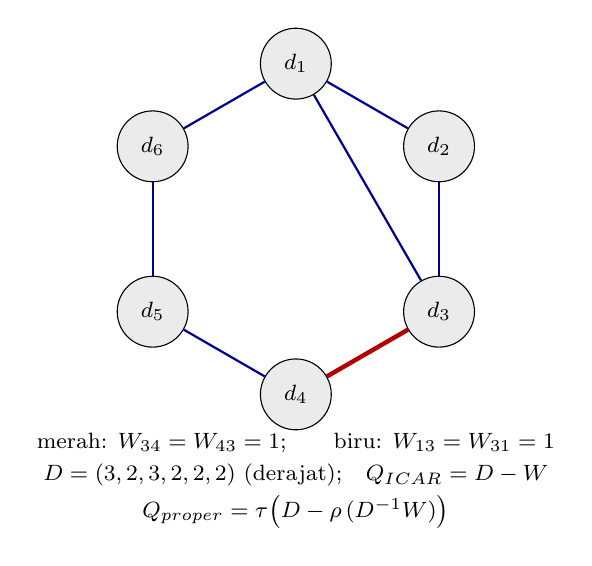
\begin{tikzpicture}[
  dom/.style={circle, draw=black, fill=black!8, minimum size=9mm,
              inner sep=1pt, font=\footnotesize},
  nbr/.style={blue!60!black, thick},
  same/.style={red!70!black, ultra thick},
  lab/.style={font=\footnotesize, align=center}]
  \node[dom] (d1) at (90:2.1)  {$d_1$};
  \node[dom] (d2) at (30:2.1)  {$d_2$};
  \node[dom] (d3) at (-30:2.1) {$d_3$};
  \node[dom] (d4) at (-90:2.1) {$d_4$};
  \node[dom] (d5) at (-150:2.1) {$d_5$};
  \node[dom] (d6) at (150:2.1) {$d_6$};
  \draw[nbr] (d1) -- (d2);
  \draw[nbr] (d2) -- (d3);
  \draw[same] (d3) -- (d4);
  \draw[nbr] (d4) -- (d5);
  \draw[nbr] (d5) -- (d6);
  \draw[nbr] (d6) -- (d1);
  \draw[nbr] (d1) -- (d3);
  \node[lab] at (0,-3.2)
    {merah: $W_{34}=W_{43}=1$;\qquad biru: $W_{13}=W_{31}=1$\\[2pt]
     $D=\diag(3,2,3,2,2,2)$ (derajat);\quad
     $Q_{\text{ICAR}}=D-W$\\[2pt]
     $Q_{\text{proper}}=\tau\bigl(D-\rho\,(D^{-1}W)\bigr)$};
\end{tikzpicture}
\caption{Graf tetangga enam domain beserta matriks yang diturunkannya.
Derajat dibaca dari graf: $d_1$ dan $d_3$ bertiga, sisanya bertua. Matriks
bobot apa pun (matrix, \code{nb}, \code{listw}) dikonversi ke graf biner
simetris oleh \code{.convert\_spatial\_weights} sebelum masuk
\code{inla.graph}. Sumber: \texttt{R/inla\_utils.R:27-88} dan pemakaian
$Q$ di \texttt{R/hb\_area.R:411-488}.}
\label{fig:neighbour}
\end{figure}

\begin{figure}[htbp]
\centering
\begin{tikzpicture}[
  lat/.style={circle, draw=blue!60!black, fill=blue!12, minimum size=9mm,
              inner sep=1pt, font=\footnotesize},
  obs/.style={circle, draw=black!70, fill=black!8, minimum size=9mm,
              inner sep=1pt, font=\footnotesize},
  arw/.style={-{Stealth[length=2.2mm]}, thick},
  dep/.style={thick, dashed, red!65!black}]
  \node[lat] (xi) at (0,1.1)   {$x_i$};
  \node[lat] (xj) at (0,-1.1)  {$x_j$};
  \node[obs] (yi) at (3.4,1.1) {$y_i$};
  \node[obs] (yj) at (3.4,-1.1) {$y_j$};
  \draw[arw] (xi) -- (yi);
  \draw[arw] (xj) -- (yj);
  \draw[dep] (xi) -- node[right, font=\footnotesize, pos=0.45]
    {$Q_{ij}\ne0$} (xj);
  \node[font=\footnotesize, align=center] at (1.7,-2.5)
    {biru = laten ($x$, GMRF); hitam = diamati ($y$)\\
     putus-putus = ketergantungan struktural};
\end{tikzpicture}
\caption{Struktur ketergantungan pada field laten GMRF: hanya pasangan
dengan $Q_{ij}\ne0$ yang bersambung (markov blanket), sementara $y_i$
bergantung pada $x_i$ lewat link. Struktur $Q$ inilah yang diisi oleh
CAR/ICAR/BYM/BYM2 pada Tabel~\ref{tab:car}. Sumber:
\eqref{eq:gmrf} dan \texttt{R/hb\_area.R:411-488}.}
\label{fig:dag}
\end{figure}

\paragraph{Peta ke bab model.} Tiga pemakaian praktis kerangka di atas
terlihat pada bagian~\ref{sec:hbarea} (pilihan \code{f(...)}, prior, dan
argumen \code{hyper}), bagian~\ref{sec:hbunit} (field laten per unit
observasi), dan bagian~\ref{sec:hbtwofold} (dua tingkat ketetanggaan);
perbedaan perilaku antar ketiganya terkumpul di \code{DISCREPANCIES.md}
bagian~F (ID \texttt{HB-1}--\texttt{HB-21}).
